\documentclass[class=article, crop=false]{standalone}
\usepackage[subpreambles=true]{standalone}
\usepackage{import}

\usepackage{tikz}
\usepackage{hyperref}

\begin{document}
[Summary of preparation]

\subsection{Computational effects}

% kell motivacio section

There are two types of programs: pure and effectful (or impure). Pure programs are ones that are independent from the environment and effectful programs are the ones that \emph{do} something in the
sense that they interact with their environment. Another way of defining pure functions is: given the definition of the function and its arguments, its result is uniquely determined.

Programs invoking computational effects such as nondeterminism, probabilistic nondeterminism, exceptions, interactive input/output or side effects all constitute as effectful. This is obvious for
interactive input/output, nondeterminism and side-effects as these obviously interact with the environment. Exceptions are a bit awkward in the sense that throwing them is pure but catching them is
not (consider catching an exception that is thrown due to an out-of-memory error; catching this exception would mean that we interact with the environment in an implicit way).

Reasoning about pure programs is easy, as pure computations (partial functions) are well understood. However, most programs must \emph{do} something with the real world (write to a file, 
read from a network socket, handle errors, generate random numbers, etc.) and perform effects to be useful.
Hence, to be able to reason about our programs we must properly understand the properties of these effects, how they work, how they interact and what rules apply to them. To do this, we try to model
them in a framework that was always know to work: mathematics.



\subsection{Eff}

This subsection gives a short introduction to Eff with some code examples. The precise syntax and semantics of the language will be defined later, we aim for an intuitive introduction here.

\subsubsection{Effects}

There is an important distinction between syntactic and semantic elements in the language. Effect declarations belong to syntax.

An effect in Eff is declared using the \verb|effect| keyword together with a type signature which forms the effect signature. One would define a \verb|Print| effect for printing strings as follows:

\begin{verbatim}
effect Print : string -> unit
\end{verbatim}

This tells us two things. To invoke the \verb|Print| effect we must provide a string as an argument and what we get back is something of type \verb|unit| after the effect is performed. We get to know no extra information about \verb|Print|.

Now that we have a \verb|Print| effect we can write down the mandatory Hello World example:
\begin{verbatim}
perform (Print "Hello World!")
\end{verbatim}

The \verb|perform| keyword is used to perform already declared effects. However, if we think about it, this piece of code still does
not make any sense as we don't know how to interpret \verb|Print "Hello World!"|.

\subsubsection{Handlers}

Handlers are used to assign meaning to effects. A handler is just a list of rules. A rule can be of three different types: a value rule, an effect rule or a finally rule.

\textbf{Value and effect rules}

The following handler provides an interpretation for the \verb|Print| effect. This handler converts the result of a computation to a 2-tuple where the first element is the original result and the second
element is a concatenation of the strings from all the \verb|Print| effects from the computation.

We use the value rule \verb|v -> (v, "")| to say what happens ``by default''. If the computation didn't print anything then we simply say that it printed the empty string.

\begin{verbatim}
let collect = handler
| v -> (v, "")
| effect (Print str) k ->
    (* Find out what the rest of the computation would print out *)
    let (result, s) = continue k () in
    (* Prefix the string printed by the rest of the computation 
       with `str` from this effect *)
    (result, str ^ s)
\end{verbatim}

The effect rule is a bit more involved. Effect rules have the form \verb|effect E(args) k| where \verb|k| is always bound to the ``rest of the computation'' which we call a continuation (and by convention
usually use the letter $k$ or $\kappa$ to denote it). The arguments of the effect \verb|E| are bound to \verb|args| via pattern matching. In the example above we first resume the computation by resuming the
computation via \verb|continue|. After we find out what the rest of the computation would print out, we prepend our current string to it.

Note that when we handle an effect of type $\alpha \to \beta$ we get a continuation of type $\beta \to \gamma$ where $\gamma$ is the type of the computation being enclosed in a \verb|with ... handle| block.

Value rules can be omitted in handler definitions, in which case they are assumed to be identities.

\textbf{Finally rules}

Finally rules are just syntactic sugar for \verb|let| wrappers around \verb|with ... handle| statements that act on the result of a handled computation, i.e.,
\begin{verbatim}
let h = handler
    | finally x -> x + x
in 
    with h handle c
\end{verbatim}
would be syntactic sugar for
\begin{verbatim}
let x = with h handle c in x + x.
\end{verbatim}

I would like to point out that this syntax is added only for convenience as it happens many times that the same transformations must be performed after a \verb|with ... handle| block \cite{bauer2015programming}. Hence \verb|finally| here does not provide the Java-like semantics where the computation in a finally block is ``guaranteed'' to be executed.

Finally rules can be omitted in handler definitions, in which case they are assumed to be identities.

\textbf{Handler types}

Handlers handling a computation of type $\alpha$ and giving a result of type $\beta$ are given the type $\alpha \Rightarrow \beta$.

\subsection{Advantages}

Now that we introduced Eff, let's switch focus and think about the programming paradigms handlers introduce.

\subsubsection{OOP and functional style}

We can think about effect signatures as interfaces and handlers as implementations of these interfaces.
A \verb|with h handle c| block is then an ``instantiation'' of effect implementations.

We see that programming with effect handlers puts us between the object-oriented and functional styles and gives us more opportunities to re-use existing pieces of code (see next code example).

\subsubsection{Direct style}

The following example shows an implementation of the state monad (borrowed from the official Eff website \cite{eff-website}):
\begin{verbatim}
effect Get: int
effect Set: int -> unit

let monad_state initial = handler
  | y -> (fun s -> (y, s))
  | effect Get k -> (fun s -> (continue k s) s)
  | effect (Set s') k -> (fun _ -> (continue k ()) s')
  | finally f -> f initial
;;

let double_and_add_ten () =
  let x = perform Get in
  perform (Set (2 * x));
  perform Get + 10
;;

with monad_state 30 handle
  double_and_add_ten ()
;;
\end{verbatim}

Note how the function \verb|double_and_add_ten| is written in a direct style. As mentioned above, the programmer does not have to 
be aware of the implementations of the effects (indeed, we see that the ``internal'' representation of state uses functions). 
This function illustrates how handlers increase the modularity of our programs (we could use the function in the context of other handlers 
and perhaps get some other result).

\subsubsection{Composition}

Monads are frequently used as a way to simulate effectful computations in programming languages like Haskell. 
However, combining different kinds of effects in these languages can be non-trivial and 
tiresome sometimes. Haskell uses monad stacks and monad transformers to get around this. [TODO: someone might not know what this is]

In Eff, combining effects and their handlers arises naturally. Handlers can be written for any set of effects and handlers can be combined 
with nesting \verb|with ... handle| blocks.

[TODO: I need two code examples here to justify the claims above and show that \verb|with ... handle| is more convenient. One in Haskell with monad transformers and one in Eff with two nested handlers.]

\subsection{Limitations}

Although there are many attractive properties of effect handlers, one that is frequently quoted to be ``annoying'' is that it is very easy to write incomprehensible code via continuations.
Continuations are not a novel concept but it is one that perhaps isn't widely known by the wider software engineering community. Hence providing the concrete implementation of effects
can impose some extra burden on a programmer's brain.


\subsection{What this dissertation is about}

Algebraic effects and their handlers lie in the heart of the Eff language.
This dissertation is concerned with building and assessing the performance of an Eff compiler.
I describe a CEK-like abstract machine in the implementation section and how that can be turned
into a more efficient Multicore OCaml-like virtual machine built on top of fibers.

This dissertation fits in the broader area of work as I hope to show that algebraic effect handlers
are not just an exciting esoteric research programming language construct with a nice theoretic background, but programming with them comes with benefits and it is possible to compile them efficiently (or at least that the cost of compilation is not too great compared to the benefits they provide).

\subsection{TODOs}
\begin{itemize}
\item I haven't said anything about continuations yet
\item I haven't said anything about shallow and deep handlers
\item Comparing to haskell monads/monad transformers is risky -- need to explain these
\end{itemize}

\section{Papers}
\begin{itemize}
\item Delimited control \cite{kiselyov2010delimited}
\item Eff Directly in OCaml \cite{Kiselyov_2018}
\item Very good article about CPS compilation \cite{flanagan1993essence}
\item Bauer tutorial \cite{bauer2018algebraic}
\end{itemize}

\section{Tikz}
\begin{figure}
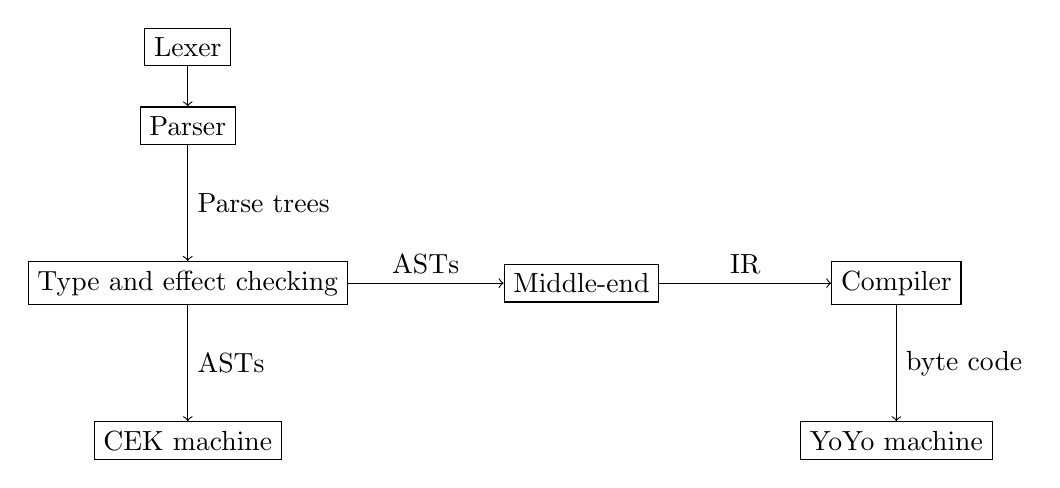
\begin{tikzpicture}
  \node[draw] (LEX) at (0,5) {Lexer};
  \node[draw] (PAR) at (0,4) {Parser};
  \node[draw] (TYPE) at (0,2) {Type and effect checking};
  \node[draw] (MID) at (5, 2) {Middle-end};
  \node[draw] (COMP) at (9,2) {Compiler};
  \node[draw] (CEK) at (0,0) {CEK machine};
  \node[draw] (YOYO) at (9,0) {YoYo machine};
  
  \draw[->] (LEX) -- (PAR);
  \draw[->] (PAR) -- (TYPE) node[midway, right] {Parse trees};
  \draw[->] (TYPE) -- (CEK) node[midway, right] {ASTs};
  \draw[->] (TYPE) -- (MID) node[midway, above] {ASTs};
  \draw[->] (MID) -- (COMP) node[midway, above] {IR};
  \draw[->] (COMP) -- (YOYO) node[midway, right] {byte code};
\end{tikzpicture}
\caption{Project structure}
\label{fig:project-structure}
\end{figure}

The project structure can be seen on \autoref{fig:project-structure}.

\end{document}